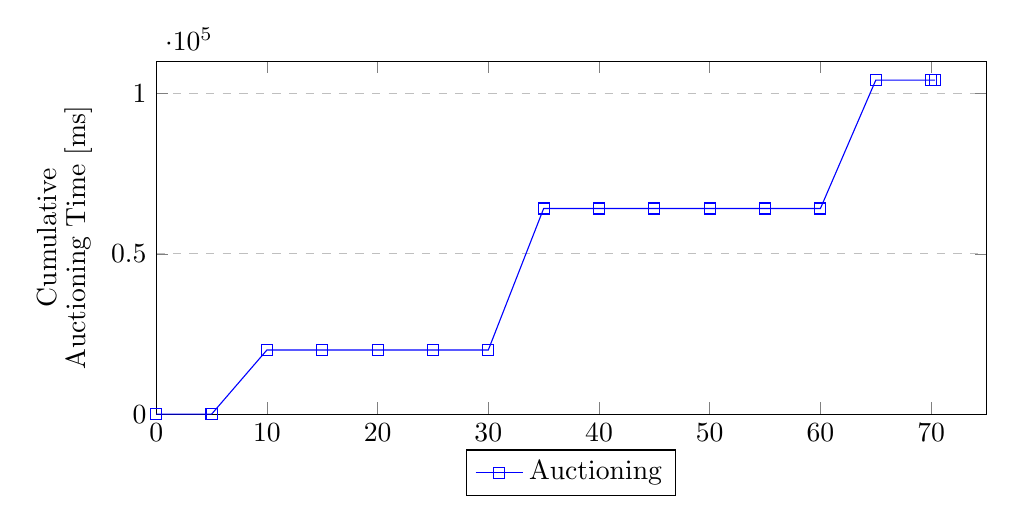
\begin{tikzpicture}
\begin{axis}[
    xlabel={Timestamp [s]},
    ylabel={\shortstack{Cumulative \\ Auctioning Time [ms]}},
    xmin=0, xmax=75000,
    ymin=0, ymax=110011,
    legend columns=-1,
    legend style={at={(0.5,-0.1)},anchor=north},
    ymajorgrids=true,
    grid style=dashed,
    width=\textwidth,
    height=0.5\textwidth,
    scaled x ticks=base 10:-3,
    xtick scale label code/.code={}
]

	\addplot[color=blue,mark=square] coordinates {
        (0,0)(5000,0)(10000,20017)(15000,20017)(20000,20017)(25000,20017)(30000,20017)(35000,64126)(40000,64126)(45000,64126)(50000,64126)(55000,64126)(60000,64126)(65000,104133)(70000,104133)(70357,104133)
    };
    \addlegendentry{Auctioning}




\end{axis}
\end{tikzpicture}